% Created 2016-09-15 Thu 10:36
\documentclass[11pt]{article}
\usepackage[utf8]{inputenc}
\usepackage[T1]{fontenc}
\usepackage{fixltx2e}
\usepackage{graphicx}
\usepackage{longtable}
\usepackage{float}
\usepackage{wrapfig}
\usepackage{rotating}
\usepackage[normalem]{ulem}
\usepackage{amsmath}
\usepackage{textcomp}
\usepackage{marvosym}
\usepackage{wasysym}
\usepackage{amssymb}
\usepackage{hyperref}
\tolerance=1000
\usepackage{listings}
\author{Daniel Dyla}
\date{\today}
\title{CSE 361 HW-1}
\hypersetup{
  pdfkeywords={},
  pdfsubject={},
  pdfcreator={Emacs 24.5.1 (Org mode 8.2.10)}}
\begin{document}

\maketitle
\tableofcontents


\section{Zero Sum Implementations}
\label{sec-1}
\subsection{Brute Force Approach}
\label{sec-1-1}

\lstset{language=Python,label= ,caption= ,numbers=none}
\begin{lstlisting}
def zerosum_brute(a):
  for i in range(len(a)-1):
    for j in range(i+1, len(a)):
      if a[i] == -a[j]:
	return((i,j))

  return (-1, -1)
\end{lstlisting}

\subsubsection{Correctness}
\label{sec-1-1-1}

The algorithm terminates because the for loops have finite bounds. The
outer loop considers every element except the last. The inner loop
checks each element against each element to its right. If the two
considered elements sum to zero we return early. If every pair is
considered without sucess we return failure.

\subsubsection{Runtime}
\label{sec-1-1-2}

\begin{align}
\sum_{i=0}^{n-2} \sum_{j=i+1}^{n-1} 1 &= \sum_{i=0}^{n-2} n - 1 - (i + 1) -1 \\
&= \sum_{i=0}^{n-2} n - i - 1 \\
&= \sum_{i=0}^{n-2} n - 1 - \sum_{i=0}^{n-2} i \\
&= (n - 2 - 0 + 1)(n-1) - \frac{(n-1)(n-2)}{2} \\
&= \Theta (n^2)
\end{align}

\subsection{Smarter Approach}
\label{sec-1-2}

\lstset{language=Python,label= ,caption= ,numbers=none}
\begin{lstlisting}
def zerosum_smarter(a):
  a = sorted(a)
  l = 0
  r = len(a)-1
  while (l < r):
    s = a[l]+a[r]
    if s == 0:
      return a[l], a[r]
    elif s < 0:
      l += 1
    elif s > 0:
      r -= 1
  return None,None
\end{lstlisting}

\subsubsection{Correctness}
\label{sec-1-2-1}

The algorithm terminates because s can only be positive, negative, or
zero. If s is 0 the algorithm returns. If s is negative l increments,
if s is positive r decrements. Eventually l must be equal to r.

If the algorithm terminates early, a match is found and returned. If s
is positive, the element at r is more positive than the element at l
is negative. Moving l will only make s further from zero so r must be
moved. Conversely, if s is negative, the element at l is more negative
than the element at r is positive and r must move. If the pointers
point at the same element then no other matches need to be checked.

\subsubsection{Runtime}
\label{sec-1-2-2}

The sort runs in $\Theta (n \lg n)$. In the worst case, $l = r$.

\begin{align}
\Theta (n \lg n) + (l - 0) + ((n-1) - r) &= \Theta (n \lg n) + l + ((n-1) - l) \\
&= \Theta (n \lg n) + l + n - 1 - l \\
&= \Theta (n \lg n) + n - 1 \\
&= \Theta (n \lg n) + \Theta (n) \\
&= \Theta (n \lg n)
\end{align}

\subsection{Smartest Approach}
\label{sec-1-3}

In the worst case the whole array must be read so no solution can be
better than $\Theta (n)$

\lstset{language=Python,label= ,caption= ,numbers=none}
\begin{lstlisting}
def zerosum_smartest(a):
  s = {}
  for i,e in enumerate(a):
    if -e in s:
      return i, s[-e]
    else:
      s[e] = i
  return None
\end{lstlisting}

\subsubsection{Correctess}
\label{sec-1-3-1}

The algorithm terminates because the for loop has a defined bound.

The algorithm checks the set of "seen elements" for its compliment. If
the complement is found, the program terminates with a match. If the
entire array has been "seen" and no matches were found, there are no
matches.

\subsubsection{Runtime}
\label{sec-1-3-2}

The for loop checks, at worst, each element once. There are $n$
elements in the array. The insertion and checking of the hash table is
a constant time operation.

\begin{align}
\sum_{i=0}^{n-1} 1 &= (n-1) - 0 + 1 \\
&= \Theta (n)
\end{align}

\section{Compare Asymptotic Runtimes}
\label{sec-2}

\subsection{Random Arrays}
\label{sec-2-1}

All algorithms as written above were tested in a python 2 environment
with random int arrays with elements from -1M to +1M of size n
from 10 to 1000000. The runtimes are shown below. Runtimes are in
milliseconds.

\begin{table}[htb]
\caption{Runtimes in milliseconds for random arrays of -1M to +1M}
\centering
\begin{tabular}{lrrrrrr}
n & 10 & 100 & 1000 & 10000 & 100000 & 1000000\\
\hline
brute & .008 & .490 & 35.619 & 209.345 & 219.296 & 248.246\\
smarter & .003 & .039 & .358 & 3.064 & 41.668 & 677.971\\
smartest & .002 & .022 & .176 & .332 & .367 & .468\\
\end{tabular}
\end{table}

Interestingly, the "smarter" algorithm actually does the worst by far
for lists with many elements. I suspect this is because the brute
algorithm found matches and returned early, where the "smarter"
algorithm had to completely sort the list before beginning processing
it.

Here is the result of another test using linear values from 10000 to
100000 and plotted. Data is not the same as the table.

\subsection{Guaranteed Worst Case}
\label{sec-2-2}

In order to test worst case (no matches) I generated the same array
sizes but used only positive numbers. This guarantees that every
incarnation of the algorithm runs in its worst possible time. Runtimes
are in milliseconds.

\begin{table}[htb]
\caption{Runtimes in milliseconds for random arrays of 0 to +1M}
\centering
\begin{tabular}{lrrrrrr}
n & 10 & 100 & 1000 & 10000 & 100000 & 1000000\\
\hline
brute & .018 & .455 & 42.74 & 3952.48 &  & \\
smarter & .004 & .033 & .428 & 4.662 & 61.941 & 911.503\\
smartest & .002 & .013 & .174 & 1.54 & 12.97 & 127.61\\
\end{tabular}
\end{table}

The final two brute cells are left blank because the computation was
infeasible on my machine (and I suspect many others as well).

Here is the result as the same linear test from above, but with
positive only arrays and smaller sizes of n due to computation

\section{Graph Comparison}
\label{sec-3}

All 3 algorithms run and plotted on a graph to compare runtimes. Note:
tests rerun with much smaller but many more n values to get better
graph data.

\begin{figure}[htb]
\centering
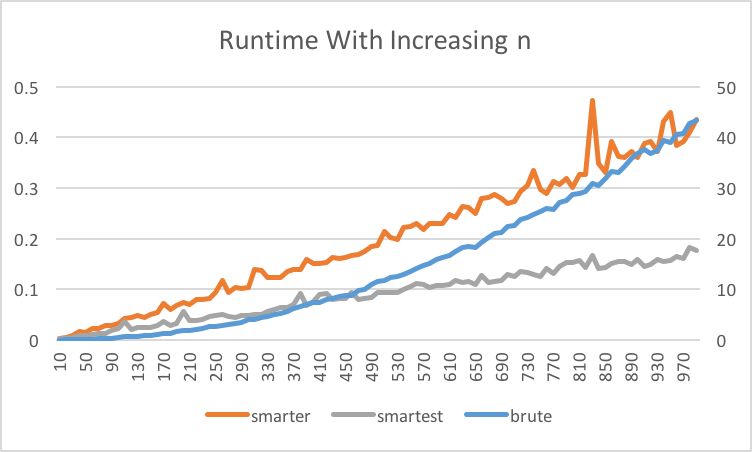
\includegraphics[width=.9\linewidth]{./hw1_graph.png}
\caption{\label{hw1_graph.png}brute algorithm plotted on secondary axis for better fit}
\end{figure}
% Emacs 24.5.1 (Org mode 8.2.10)
\end{document}
